\section{Implementierung des Senders}
\label{sec:imp_des_transmitters}
Abb.~\ref{fig:transmitter} zeigt einen funktionsfähigen DAB Sender im GRC. Der Sender transportiert zwei Audio Kanäle im MSC, wobei der obere Kanal DAB+ (MPEG4 und Reed Solomon Encoder) und der untere Kanal DAB (MPEG 2 Encoder) transportiert. Jeder Block in der grafischen Ansicht entspricht einer eigenständigen Klasse, wobei die Kanalcodierer des FIC und MSC sowie der OFDM Modulator hierarchische Blöcke sind, also mehrere Blöcke in sich zusammenfassen. Die Struktur der Blöcke als einzelne Funktionseinheiten ist von der Aufteilung dem DAB Standard nachempfunden. Bei der Implementierung wurde darauf geachtet, möglichst viel Funktionalität in eine Klasse zu integrieren ohne dabei an Flexibilität der Blöcke einzusparen.

\begin{figure}[ht]
\centering
  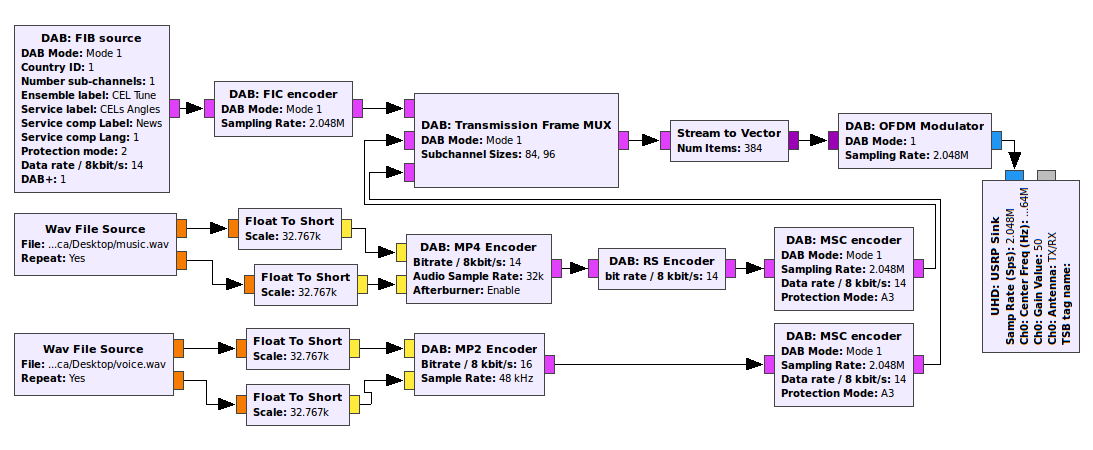
\includegraphics[width=\textwidth]{figures/GRC_transmitter.png}
	\caption{DAB/DAB+ Sender im GRC}
	\label{fig:transmitter}
\end{figure}

\subsection{FIB Quelle}
Die FIB Quelle produziert standardkonforme FIBs für den FIC. Die \ac{MCI} und \ac{SI} werden der Klasse dabei als Argumente übergeben. Die folgenden Informationen werden gesendet:
\begin{itemize}
\item Ensemble Infos: Country ID, Ensemble ID, CIF Zähler
\item Service Organisation: Country ID, Anzahl der Services, Servicebeschreibung
\item Service Component Beschreibung: sub-channel ID, Audio Typ, primary/secondary
\item Sub-channel Organistaion: sub-channel ID, Start und Länge (in CUs), Protection Mode
\item Labels für das Ensemble und jeden Service und deren Sprache (SI)
\end{itemize}
Diese Informationen umfassen bei weitem nicht das ganze Spektrum der möglichen Informationen. Sie sind aber ausreichend um dem Empfänger die nötigen MCI für die Decodierung und dem Nutzer die Informationen zur Identifikation des Programmes zur Verfügung zu stellen. Weil die MCI eine weit höhere Wichtigkeit als die SI einnimmt, wird sie mit jedem CIF geschickt. Die Größe der gesamten MCI hängt von der Anzahl der verwendeten Services und Service Komponenten ab. Bei einer Begrenzung auf maximal 7 Services mit je einem sub-channel kann die Information in den ersten zwei FIBs gespeichert werden. Im dritten FIB wird dann die SI gesendet. Da ein Label mit 16 Buchstaben ein FIB schon nahezu füllt, werden die einzelnen Labels nacheinander jeweils im dritten FIB verschickt. Dies ist nicht problematisch, da die Labels im Regelfall über die Zeit konstant bleiben und durch eine CIF Rate von $\frac{1}{24 ms} > 41 \: \text{CIFs}/s$ trotzdem jedes Label mehrmals pro Sekunde gesendet wird. \todo{evt grafik wie in blogpost week 02}

\subsection{FIC Encoder}
\label{sec:fic_encoder}
Der FIC Encoder ist in einem hierarchischen Block (Abb.~\ref{fig:fic_encoder}) implementiert. Er enthält die gesamte Kanalcodierungskette aus Kap.~\ref{sec:FIC}. Während für die CRC Berechnung und die Faltungscodierung eine jeweilige Klasse implementiert wurde, besteht die Energieverwischung, wie in Gl.~\ref{eq:energy_dispersal} beschrieben, lediglich aus einer XOR Verknüpfung des Bitstreams mit der PRBS Folge.

\begin{figure}[ht]
\centering
  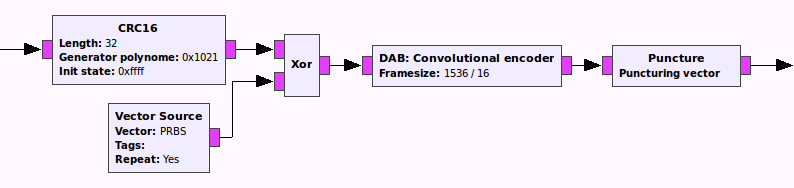
\includegraphics[width=\textwidth]{figures/FIC_encoder.png}
	\caption{Kanalcodierung im hierarchischen Block des FIC Encoders}
	\label{fig:fic_encoder}
\end{figure}

\subsection{Audio Quellen und Encoder}
Die Audioeingangsdaten der Audioencoder sind 16 bit PCM Samples. Um diese für den Stream zur Verfügung zu stellen gibt es verschiedene Möglichkeiten. Entweder werden die Audiosamples über eine Binärdatei als Rohdatenquelle zur Verfügung gestellt. Eine andere Möglichkeit bietet der "WAV File Source" Block von GNU Radio, der aus dem populären "WAVE" Audioformat die Rohdaten extrahiert und somit auch eine PCM Quelle darstellt. Eine letzte Möglichkeit ist die direkte Generation von PCM Samples über die lokale Soundkarte. Alle drei Möglichkeiten resultieren letztendlich in einem Stream mit 16 bit Gleitkommawerten, dessen Samplingrate der Audiorate entspricht. Weil die implementierten Audiocodecs auf Integerebene arbeiten, wird der Stream vor der Encodierung auf den neuen Wertebereich abgebildet.

\subsubsection{MPEG 1/2 Audio Layer II Encoder (DAB)}
Der MPEG 2 Encoder Block verwendet einen Patch der frei verfügbare mp2 Encoder Bibliothek TooLAME. Der Patch stammt vom ODR mmbTools Projekt und ist speziell auf DAB angepasst. Der Code wurde in einen GNU Radio Block gepackt um ihn in einen GNU Radio Flowgraph einzubauen. Die Funktionalität des Encoder Blocks kann mit einem Loopback-Test verifiziert werden, indem der encodierte Stream mit einem Audio-Player erfolgreich decodiert und abgespielt wird.

\subsubsection{MPEG 4 HE-AACv2 (DAB+)}
Der MPEG 4 Encoder basiert auf einem Patch der FDK-AAC Codec Bibliothek für Android der Fraunhofer-Gesellschaft zur Förderung der angewandten Forschung e.V.. Die Bibliothek untersützt eine Reihe von AOTs (Audio Optimization Tools) welche die Audiokompression nach unterschiedlichen Paramtern optimieren. Es stehen die folgenden AOTs zur Verfügung:
\begin{itemize}
\item AAC-LC: Geringe Komplexität ($1,5$ bits/sample) für minimales Codierungsdelay
\item HE-AAC Dualband SBR: Hohe Effizienz ($0,625$ bits/sample) durch Spektralbandreplikation.
\item HE-AAC v2 PS: Zusätzlich mit paramterisiertem Stereo ($0,5$ bits/sample)
\end{itemize}
Ein Patch des "ODR-AudioEnc" Moduls wurde für die Implementierung des GNU Radio Blocks genutzt.\\
DAB+ enthält neben der neuen Audiokompression eine zusätzliche Fehlerkorrektur durch einen Reed-Solomon Code. Um den MPEG 4 Encoder Block nicht zu sehr auf DAB+ zu spezialisieren, wurde der Reed-Solomon Encoder in einem separaten Block Implementiert.

\subsection{MSC Encoder}
Der MSC Encoder entpricht von Aufbau und Struktur dem FIC Encoder Block aus \ref{sec:fic_encoder}. Der Block enthält eine zusätzliche Klasse für das Zeitinterleaving und besitzt keinen CRC Generator.

\subsection{Multiplexer}
Der Multiplexer Block hat prinzipiell die Aufgabe eines Parallel-Seriell Wandlers. Er besitzt $1 +$ \# sub-channels Eingänge und setzt diese zu einem Sendesignale nach der Struktur aus~\ref{sec:transmission_frame} zusammen. Die Position der jeweiligen Audiostreams im CIF werden dabei über die selbe MCI bestimmt, die in den FIBs des FIC desselben Sendeframes stehen. Die Synchronisationssymbole $z_{0,k} \text{und} z_{1,k}$ sind an dieser Stelle noch nicht vorhanden und werden dem Sendeframe im OFDM Modulator hinzugefügt.

\subsection{OFDM Modulator}
Der OFDM Modulator Block ist ein hierarchischer Block mit vielen Unterklassen. Jede Klasse führt dabei einen der in \ref{sec:ofdm_mod} beschriebenen Schritte zur Modulation durch.

\subsubsection{QPSK Mapping}
Der QPSK Mapper bildet 1 Byte auf 4 komplexe QPSK Symbole ab. Da wie in \ref{sec:qpsk} beschrieben zuerst die Realteile und anschließend die Imaginärteile eines kompletten OFDM Symbols übertragen werden, kann der QPSK Mapper nicht einfach im Streammodus arbeiten, also jedes Byte direkt auf 4 QPSK Symbole abbilden. Ein Gedächtnis der Klasse kostet Rechenzeit, weil die Eingangsdaten zusätzlich einmal ins Gedächtnis kopiert werden müssen. Um dies zu vermeiden arbeitet der Mapper auf Vektorbasis der Länge $1536/4$ Bits am Eingang, bzw. $1536$ Bits am Ausgang. Dies umfasst genau der Länge eines OFDM Symbols.

\subsubsection{Einfügen des Phasenreferenzsymbols}
Das Phasenreferenzsymbol wird schon als QPSK Symbol (um $\pi/4$ gedreht) generiert. Daher wird es erst nach der QPSK Modulation der Datensymbole an das Sendeframe angehängt. Das Phasenreferenzsymbol ist bei jedem Sendeframe gleich und kann deshalb im Konstruktur einmalig generiert werden.
\subsubsection{Differentielle Modulation}
Die Differentielle Modulation stellt eine einfache komplexe Multiplikation eines jeden Symbols mit dessen Vorgänger dar (siehe~\ref{sec:diff_mod}. Auch hier wird auf Vektorbasis gearbeitet.

\subsubsection{Frequenzinterleaving}

\subsubsection{\ac{IFFT}}
Die OFDM Operation kann nach~\ref{sec:ofdm} als \ac{IDFT} durchgeführt werden. Ein Teil der $N=2048$ Unterträger sind nicht belegt. Diese müssen vor der Transformation als komplexe Nullsymbole eingefügt werden. Wegen $2048 = 2^{11}$ kann die IDFT als eine deutlich schnellere IFFT realisert werden. Ein IFFT Block ist im GNU Radio Modul gr-fft\todo{cite properly} vorhanden.

\subsubsection{Einfügen des Cyclic Prefixes}
Nach der IFFT liegt das Sendesignal nun im Zeitbereich vor. Das Einfügen des Cyclic Prefixes entspricht dem Kopieren vom Ende jedes Symbols an den Anfang. Das Einfügen eines Cyclic Prefixes ist eine weitverbreitete Technik bei OFDM. Daher existiert in GNU Radio schon ein Block mit dieser Funktionalität, der nur noch mit der passenden Symbollänge $T_S = 2048$ Samples und der Länge des Cyclic Prefixes $T_G = 504$ Samples initialisiert werden muss.

\subsubsection{Einfügen des Nullsymbols}
Als letzter Schritt in der Sendekette erfolgt das Einfügen des Nullsymbols. Dabei werden $T_{NULL}=2656$ Samples mit dem Wert $0+0j$ zwischen zwei Sendeframes geschrieben.

\subsubsection{}
Das Basisbandsignal ist nun bereit um hochgemischt und anschließend gesendet zu werden. Beide Schritte sind in dem GNU Radio Block USRP Sink vereint. Alternativ lässt sich das Basisbandsignal natürlich auch als I/Q Daten in einer Binärdatei speichern.